\documentclass{sig-alternate}
\def\allfiles{}
\usepackage{latexsym}
\usepackage{amsmath}
\usepackage{algorithm,algorithmic}
\usepackage{graphicx}
\usepackage{url}
\usepackage{subfigure}

\title{Extracting User's Hidden Profile on Twitter}

\author{Dong Wang, Mohan Yang, Yuchen Liu}

\begin{document}

\maketitle

\begin{abstract}
Targeting user profile to match a user with specific services is a fundamental task for social network system. In this paper we are given a set of users within a category $\mathcal{C}$ and would like to infer which users are also in this category with high probability. We show that the information contained in graph structure and tweets are highly related to users profile. We develop several algorithms and design the co-training framework based on bidirectional snowball algorithm and naive Bayes algorithm. Our experiments on Twitter social network show that our approaches performs well in retrieving users within target category.
\end{abstract}

\section{Introduction}

Twitter, a micro-blogging system combining social network and text content, has demonstrated itself as a leading breaking news provider, and a platform of sharing opinions and interests. The text content published by users is called tweet, which is within 140 characters in length. Common practice of responding to a tweet includes retweet a tweet, like a tweet and reply a tweet. Users are connected with each other by the following relation. Following a user means subscribing to his tweets as a follower. This does not require other user's permission. A user can follow any other users, but others are not required to follow back. This non-reciprocal relation is much different from the friend relation in social networking services like Facebook and MySpace.
User on Facebook has a complete profile by filling out his education, work and interest, while Twitter user can only fill out a piece of 160 characters bio information. It is difficult to precisely recommend related users, news and services on Twitter with limited user profile information. Thus, extracting a user's hidden profile is a valuable topic which improves user experience and advertisement revenue at the same time. Additionally, it will also help to improve the search result relevance by assigning a higher rank to the results in which the user is more interested.
We will propose an algorithm to extract a user's hidden profile from his followers and followings using the closeness and tweets similarity of two users, which is based on the intuition that people with similar background and interests tend to connect with each other.
However, proposing an efficient solution to the problem is very challenging due to sparseness and incompleteness of the following relation data. The Twitter network graph is a very large but spare graph which involves over a hundred million users, while most of them are connected to only hundreds of users. Additionally, some users have more than a thousand followers which cannot be completely retrieved due to the limit of Twitter API. Thus, our algorithm should be able to predict with sparse and incomplete following relation data.


\subsection{Paper Organization}

The rest of the paper is organized as follows.  Section
\ref{sec:related-work} compares our work with related work.  Section
\ref{sec:problem} presents the mathematical formulation of the
problem.  Section \ref{sec:method} presents

\ifx \allfiles \undefined
\documentclass{article}
\usepackage{booktabs}
\usepackage{multirow}
\usepackage{graphicx}

\begin{document}
\title{Problem Formulation}
\maketitle \else \fi

\newcommand{\following}{\ensuremath{following}}
\newcommand{\follower}{\ensuremath{follower}}

\section{Problem Formulation}\label{sec:problem}
We formulate the social network in twitter as a directed graph $G = (V,E)$.
Each node $u \in V$ represents a user in twitter, and a directed edge $(u,v) \in E$ indicates
user $u$ is following user $v$. The set of users who are following user $u$ is denoted as $\follower(u)$, and the set of users followed by $u$ is denoted as $\following(u)$. The size of these two sets are $|\follower(u)|$ and $|\following(u)|$, respectively.

For each individual user $u$, we collected the user's tweets
$T(u)=\{t_1, t_2, \cdots\}$.
Each tweet contains a set of words in $W=\{w_1, w_2, \cdots\}$.
We use a vector $\phi_u$ represents the word feature generated by the user.
Here $\phi_{u,i}=1$ indicates that word $w_i$ appeared in $u$'s tweets,
and $\phi_{u,i}=0$ indicates that word $w_i$ did not appeared in $u$'s tweets.
To simplify our problem, we ignore the number of occurrences of each word $w_i$.

In addition to a user's short bio,
we also collected a series of characteristic keywords
$z_1, z_2, \cdots$ from his short bio. For example, a student study computer
science in UCLA may write ``Computer science student at UCLA'' in his short bio.
We extract his characteristic profile as
$z_1=$Computer Science, $z_2$=student, $z_3=$UCLA.
Because computer could not generate these characteristic profile automatically
and accurately, we choose some phrases manually and consider other words in
profile as single keyword for the user.

Given a keyword or phrase $z_i$, we call users which write $z_i$ in their
short bio directly as nodes $L={l_1, l_2, \cdots, l_n}$,
while we call other users without the $p_i$ as nodes $D={d_1, d_2, \cdots, d_m}$.
The total user set we have is $C=D \cup L$.
Although some users in nodes set $D$ have not write $p_i$ in their profile,
he actually owns the keyword or phrase in real life.
As the example before, a student in UCLA could also write
``loving being a BRUIN and loving God!'' in her short bio.

Now our task is to design some algorithms that for a specify keyword or
phrase $z_i$, predict how user $u$ in nodes set $D$ is related with $z_i$.
In order to achieve this goal, we may assign some weight on words appeared
in user's tweets, short bio, or locations. Additionally, we may analysis
user's link relationship with others.
Our result would be a sorted list that ranks the user with high probability
having $z_i$ in real life at first.

\ifx \allfiles \undefined
\end{document}
\fi

\ifx \allfiles \undefined
\documentclass{article}
\usepackage{booktabs}
\usepackage{multirow}
\usepackage{graphicx}

\begin{document}
\title{Method}

\newcommand{\following}{\ensuremath{following}}
\newcommand{\follower}{\ensuremath{follower}}

\maketitle \else \fi

\newcommand{\argmax}{\operatornamewithlimits{argmax}}

\section{Our Approach}\label{sec:method}

\subsection{Snowball Algorithm}
%In considering the operational models for the extraction of a profile keyword of a user through a social network $G$, we will first treat this problem as an information influence spread processing.

Given a category $\mathcal{C}$ and a keyword $z_{\mathcal{C}}$ which best describes $\mathcal{C}$, each user $u \in V$ has an active score $s_u$ representing the likelihood that $u$ belongs to category $\mathcal{C}$. If $s_u \geq 1$, user $u$ is \emph{active}, indicating $u$ belongs to $\mathcal{C}$; otherwise, $u$ is \emph{inactive}. The snowball algorithm calculates $s_u$ based on the linear threshold model proposed in \cite{snowball1,snowball2}, which captures the influence propagation process in the network.

%For more information, please view paper Maximizing the spread of influence through a social network, page 2.

%Given keyword $z_{\mathcal{C}}$, users are partitioned into sets $\mathcal{A}$ and $\mathcal{B}$. The users in $\mathcal{A}$ are active, and users in set $\mathcal{B}$ are inactive. We focus on settings guided by previous work about the spread of influence in which each user's state to become active increases monotonically as more of its friends become actives. The snowball algorithm is an iterative algorithm. Once a user become active, it remains active in the future iterations. For an inactive user $u$, more and more followings of $u$ become active after many iterations, and $u$ might become active if enough
%as time passed, more and more of users followed by $u$ become active; at some point, this cause $u$ to become active, and $u$ influenced his followers.

As shown in Algorithm~\ref{alg:snowball}, the snowball algorithm is an iterative algorithm. Initially, the active score of users in $\mathcal{A}$ is set to 1, while the active score of users in $\mathcal{B}$ is set to 0. So only users in $\mathcal{A}$ are active at the beginning. During each iteration, the algorithm scans through each inactive user $u$ and calculate its new active score based on the active score of $u$'s followings:
\begin{equation}\label{eq:snowball}
s_u = \sum_{v \in \following(u)} \frac{s_v}{|\follower(v)|}
\end{equation}
If the new active score $s_u$ is no less than 1, then user $u$ becomes active. Although user $u$ is inactive at the beginning, he might become active as many of his following becomes active during the iteration, and he will be able to contribute to his followers once he becomes active. The algorithm iterates until no more users could become active. Users in $\mathcal{B}$ are ranked based on the time at which they become active.
%In order to obtain the ranking result for $z_{\mathcal{C}}$, here we rank the inactive users in $D$ according to their time point to become an active user.

%------------------------------------------------
\begin{algorithm}[htbp]
\caption{\textsc{Snowball}}
\textbf{Input: }{Category $\mathcal{C}$ and keyword $z_{\mathcal{C}}$}\\
\textbf{Output: }{An array $rank$ containing the users in $\mathcal{B}$ ranked on the probability of belonging to $\mathcal{C}$}
\begin{algorithmic}[1]
\STATE $s_u \leftarrow 1$ {\bf for} $u \in \mathcal{A}$, $s_u \leftarrow 0$ {\bf for} $u \in \mathcal{B}$
\WHILE{$rank$ changed during last iteration}
\FOR{$u \in V$ s.t. $s_u < 1$}
    \STATE update $s_u$ according to Eqn.~(\ref{eq:snowball})
    \STATE {\bf if} $s_u \geq 1$, {\bf then} add $u$ to $rank$
\ENDFOR
\ENDWHILE
\STATE {\bf for} $u \in V$ s.t. $s_u < 1$ {\bf do} add $u$ to $rank$
\RETURN $rank$
\end{algorithmic}
\label{alg:snowball}
\end{algorithm}
%------------------------------------------------

\subsection{Bidirectional Snowball Algorithm}

The underlying graph structure of twitter social network is similar to that of the Web graph, where a user in twitter corresponds to a page in the Web, and a following relation between two users corresponds to a directed hyperlink between two pages. Existing methods like PageRank\cite{page1999pagerank}, TrustRank\cite{gyngyi2004combating} and random walks with restarts\cite{tong2006fast} are popular random walk based methods for ranking nodes in the Web graph. Our second approach uses a variant of TrustRank to calculate the relevance score $s_u$ for each user $u$. The idea is user $v$ positively contributes to $u$'s relevance score if $v$ is $u$'s following, and user $w$ also positively contributes to $u$'s relevance score if $w$ is $u$'s follower.

%Considering the graph structure generated by twitter social network, it is similar to web graph structure where users are pages, and there are some outgoing links from $u$ to $v$ since that $u$ is following $v$, and also incoming links from $v$ to $u$ since that $u$ is followed by $v$.

%In order to predict the relationship between keywords or phrase and users, a second general approach is to predict the relationship importance between users in $D$ and users in $L$. For user $u$, an easy way to rank the importance of other users to him is performing the random walk from $u$. After the random walk starting from user $u$ go through his friends links, we obtain the rank of users in which top ranked users might be most important guy that $u$ follows. By the random walk starting from user $u$ go through his follower links, we obtain the rank of users in which top ranked users might be most important guy that followed $u$. For a specified or phrase $z$, we add undirected links from $z$ to users have this keyword. And then, after the random walk from user $u$, we get how important that $z$ is related to $u$ in both directions.

Define two vectors, $P = (p_1, \cdots, p_n)$ and $Q = (q_1, \cdots, q_n)$, where $p_u$ represents the relevance score of user $u$ to category $\mathcal{C}$ with respect to the following direction, and $q_u$ represents the relevance score with respect to the follower direction.
%However, we don't have computation power to perform this random walk since that there are too many users in social network. We modify this model in reverse direction as the Trust-rank algorithm. For keyword or phrase $z_i$, we use $a_j$ represent the importance that user $u_j$ is related to $z_i$ in friends direction and $s_j$ represent the importance that $u_j$ is related to $z_i$ in followers direction. Additionally, we use vector $P = (p_1, p_2, \cdots, p_n)$ and $Q = (q_1, q_2, \cdots, q_n)$.
In the following direction, $u$ receives weight from each of his followings with probability $(1 - d) / |\following(u)|$. On the other hand, $u$ receives weight from each of his followers with probability $(1 - d) / |\follower(u)|$ in the follower direction. The random walk is formulated as:
\begin{eqnarray}\label{eq:randomwalk}
P & = & (1 - d) M_P P + d T \nonumber \\
Q & = & (1 - d) M_Q Q + d T
\end{eqnarray}
$M_P$ and $M_Q$ are $n \times n$ transition matrices described above. Vector $T$ represents the trust value of each user, where $T_u = \frac{1}{|\mathcal{A}|}$ for $u \in \mathcal{A}$ and $T_u = 0$ for $u \in \mathcal{B}$. $d$ is the damping factor.

The initial value of $p_u$ and $q_u$ is ${1 \over |\mathcal{A}|}$ for $u \in \mathcal{A}$, otherwise it is 0. Each iteration updates the value of $P$ and $Q$ based on Eqn.~(\ref{eq:randomwalk}), and normalizes vector $P$ and $Q$ into unit vectors. Finally, the users are ranked according to the relevance score $s_u = p_u q_u$ after convergence, which is a combination of relevance to category $\mathcal{C}$ from both following and follower directions.

\subsection{Naive Bayes Algorithm}

The above two algorithms works well in many situations. However, the tweets information are ignored in these two approaches. Our third approach builds a classifier using the tweets information, and predicts how likely a user in $\mathcal{B}$ belongs to category $\mathcal{C}$. The users in $\mathcal{A}$ are positive training examples, and the users in $\mathcal{B}$ are negative training examples.

%Both two models described above works well in some situations. However, we ignore the tweets information and other profile information in our dataset. With the information extracted from our dataset, another general approach to our problem would be to view it as a classification task. We take users that already have some profile keyword as positive training examples, and treat other users as negative training examples. Then we could learn a classifier that predicts how likely that a user is going to have a profile keyword.

There are many machine learning algorithms which address this classification problem. We use the naive Bayes classifier \cite{frank2000technical} which is one of the most effective and efficient classification algorithm. The problem has two classes, class 1 and class 0. Users in class 1 belong to $\mathcal{C}$, while the users in class 0 do not belong to $\mathcal{C}$. $c = i$ represents the event that the class is $i$.

For each user $u$, let $T_u$ be the collection of $u$'s tweets, location and biography. The word set for corpus $\bigcup_{u = 1}^n T_u$ is $W = \{w_1, \cdots, w_m\}$.
%the set of tweets published by $u$ be $T_u = \{t_1, t_2, \cdots\}$, where each tweet $t_i \in T_u$ contains a set of words from $W = \{w_1, \cdots, w_m\}$. Then $T_u$ can be viewed as a bag of words from $W$.
$\mathbf{1}_{T_u}(w_i)$ is the indicator function of $T_u$, where $\mathbf{1}_{T_u}(w_i)$ equals to 1 if word $w_i$ appears in $T_u$, otherwise it equals to 0. Let $w_i = 1$ represents the event that word $w_i$ occurs, and $w_i = 0$ represents the event that word $w_i$ does not occur.

The naive Bayes classifier for $u$ tries to find $i \in \{0, 1\}$, such that
$$p(c=i | w_1 = \mathbf{1}_{T_u}(w_1), \cdots, w_m = \mathbf{1}_{T_u}(w_m))$$
is maximized, or equivalently maximize
$$p(c = i) \prod_{j=1}^m p(w_j = \mathbf{1}_{T_u}(w_j) | c = i).$$
As the problem has only two classes, it is equivalent to determining the sign for $s_u$:
\begin{eqnarray}
s_u & = & \log(p(c = 1)) - \log(p(c = 0)) \nonumber \\
    & + & \sum_{j=1}^m (p(w_j = \mathbf{1}_{T_u}(w_j)|c = 1) - p(w_j = \mathbf{1}_{T_u}(w_j)|c = 0)). \nonumber
\end{eqnarray}
The larger the value (positive value) of $s_u$, the more likely $u$ belongs to $\mathcal{C}$; the smaller the value (negative value), the more likely $u$ does not belong to $\mathcal{C}$. The value of $p(c = 1)$ is calculated as the fraction of positive training examples, and the value of $p(w_j = \mathbf{1}_{T_u}(w_j)|c = 1)$ is calculated as the number of positive examples such that $w_j$ appears (does not appear) in $T_u$ divided by the number of positive examples if $\mathbf{1}_{T_u}(w_j) = 1$ (if $\mathbf{1}_{T_u}(w_j) = 0$). The calculation of $p(c = 0)$ and $p(w_j = \mathbf{1}_{T_u}(w_j)|c = 0)$ are similar. Finally, the users in $\mathcal{B}$ are ranked based on the value of $s_u$.
%In this algorithm, the learner attempts to construct a classifier for a set of labeled training examples.
%There are several machine learning algorithms that address this problem. Here we use a Naive Bayes model which is one of the most effective and efficient classification algorithm. In this algorithm, the learner attempts to construct a classifier for a set of training example with class labels.

%Assume that $X_1, X_2, \cdots X_n$ are training vectors $X_i=(x_1, x_2, \cdots, x_m)$ and each training vector has a class label $c$. The Bayes estimate $p(x_j|c)$ from the training examples to maximize the probability:
%$$\prod_i p(c)\prod_jp(x_j|c)$$

%In our paper, we apply this Naive Bayes method to learn the probability that user $u_j$ has the profile $z_i$. And return the sorted list according the probability.

%The first is that the class is imbalance, for each profile $z_i$, there will be a very small fraction of the users in the network and learning is particularly hard in domains with high class imbalance. The second challenge is that there are huge amount of features. There are lots different words appeared in users tweets and also typos and connected words. Therefore, we modify the Naive Bayes algorithm so that for each profile keyword $z_i$, the learner could give user relevant score according to:
%We modify the Naive Bayes algorithm to calculate the relevant score according to the following equation:
%\begin{equation}
%r = \frac{1}{n_i}\sum_{i=1}^{n_i} \log p(c|w_i)
%\end{equation}

\subsection{Co-training Algorithm}

%The random walk model works well for profile which users with this profile like connected with each other. For example, users in same companies or universities would like to follow each other. The Naive Bayes model works well for profile which users with this profile like to talk about same topics. For example, users like comic probably didn't know each other and follow each, but they tweet same words for same topic.

%There is a general approach to combine two different models together and generate better result for different kind of profile keyword.
The bidirectional snowball algorithm and naive Bayes algorithm focus on different perspective of twitter networks: the former focus on the network structure level, and the later focus on the tweets information level. Both of them provide reasonably well rankings for the training data, while the perspectives of these two algorithms are conditionally independent given the ranking. A more powerful approach called co-training \cite{cotraining} combines the two algorithms together, and iteratively reinforce the result of one algorithm by the the result of the other algorithm.

%Because our two models (i) based on different prospective of user behaviors; (ii) each training method is sufficient to train a good ranker when we have enough training data; (iii) two prospective of user behaviors are conditionally independent given the class. So we use co-training \cite{cotraining} method to combine two approaches.

Let $l$ are $k$ be positive integers, and $k > l$. During each iteration, top $l$ users generated by the naive Bayes algorithm are merged into set $\mathcal{A}$ in the bidirectional snowball algorithm, and the top $l$ users generated by the new bidirectional snowball algorithm is considered as positive training examples in the naive Bayes algorithm. The iteration is executed until the top $k$ users generated by the bidirectional snowball algorithm and naive Bayes algorithm are the same. The result of the last execution of the naive Bayes algorithm is used as the final result of the co-training algorithm.

%We arrive at Algorithm 4 that iteratively computes the vector $P$, $Q$ as well as the relevant score $s_u$.
%I will write sudo code here

\ifx \allfiles \undefined
\end{document}
\fi

\ifx \allfiles \undefined
\documentclass{article}
\usepackage{booktabs}
\usepackage{multirow}
\usepackage{graphicx}

\begin{document}
\title{Method}
\maketitle \else \fi

\section{Experiments}\label{sec:experiment}
In this section, we test our different models on real dataset extracted from twitter. We name snowball algorithm as SA, random surfing algorithm as RSA, naive bayes algorithm as NBA and the combination of random surfing algorithm and naive bayes algorithm as CM. In the experiments, we use precision at the position $K$ to evaluate the accuracy of our ranking result. The precision at the position $K$ measures how many related user we ranked in top $K$ positions, thus it penalizes the model which performs poorly in top positions. Here we didn't use recall as one of our metrics since that we can hardly obtain the exactly number of users belong to our target category.

\subsection{Experimental Setup}
\textbf{User data:} The users used to train and evaluate our algorithm are collected from twitter during October, 2011. As described in section TODO, we collected TODO users from our seeds users. For each user, we also collected his at most 20 tweets in October, his profile and his followings. Thus, in total we have TODO tweets with more than TODO different words. Since user word pairs are very sparse and some word appeared in only a few users are not generalizable, we eliminate the words appeared less than 100 times and there is TODO word left.

\textbf{Label data:} During our experiments, we mainly focus on predicting users from four categories, they are UCLA, Stanford, MIT and USC. The user belong to these four universities may highly connected with each other. Later in our experiments part, we will prove that some of our algorithm will still have good performance with dataset that is not highly connected. For category of each university, we use $80\%$ users with target keyword in their short bio as training data and erase the target keyword appeared in other $20\%$ users. In the evaluation process, we will also label top TODO results by human in order to obtain a more accuracy evaluation result.

\subsection{Ranking Performance}
In this part of the experiments, we use our label data and sort the users with respect to the estimated relevance given by our algorithm. We show the detailed precision curve (at different position) for different categories in Figure TODO.

From Figure TODO we can see that the TODO and TODO performs the best at all most every positions. This fact demonstrates that TODO. Note that much of the improvement in the precision curve comes in the area near the position TODO to TODO. This is the area that we most care about, since that users in top positions have some features that is extremely easy to discover and users in these middle positions reflect the effectiveness of our algorithm more clearly.

We also show some really related users and unrelated users ranked by our algorithm in top positions in Table TODO. This table reflects our program's strengths and weaknesses. The SA TODO. The RSA TODO. The NBA TODO. The CM TODO.

Moreover, we show some of the features importance of NBA in table TODO. We ranked features according to their weight $\log p(c|w)$ and pick up the top $10$ words for different categories. From the table, we could learn some different attributes related to particular category of users. For example, UCLA students like ``dailybruin'' news, call themselves as ``bruins'' and lived near ``westwood''; USC students like news from ``usc annenberge'' and the idol statue in their university is ``Trojan''; MIT students live in ``Cambridge'' and there is famous ``media lab'' in their computer science department; Stanford students TODO.

ucla
1. dailybruin
2. bruin
3. bruins
4. westwood
5. neuheisel
6. alumna
7. wooden
8. undergraduate
9. midterms
10. royce

usc
1. ascj
2. uscedu
3. annenberg
4. uscpsycho
5. uscannenberg
6. ausc
7. beattheirish
8. trojan
9. trojans
10. atrojan

mit
1. sloan
2. medialab
3. cambridge
4. joi
5. kayak
6. bostonupdate
7. alums
8. mechanical
9. techreview
10. edu

stanford
1. stanfordfball
2. gostanford
3. astanford
4. gsb
5. cardinal
6. cantor
7. tristanwalker
8. auditorium
9. alums
10. freshmen

\subsection{Ranking with Loss of Information}
In this part of the experiments, we evaluate our different models with the loss of information. The loss of information means that during the training process, we erase some users profile in label data and treat these users as normal users without our target profile keywords. We test our program and plot the results for different amount of training data in Figure TODO.

The results show that with the loss of information, the performance of SA algorithm and RSA algorithm falls down dramatically since that the prediction based in these algorithms mainly based on graph structure and link relationship between label users. The NBA TODO. As we expect that CM algorithm TODO.

In our original dataset, the training users are likely to connected with each other since they are in same university. However, for other categories such as father, gamer or phd, users belong to such categories maybe not likely to connected with others in same category. When we erase the profile keyword in label data, the connection in label data become smaller and the structure may like other categories. The performance of our algorithms also demonstrate that our algorithms could be applied to different categories.

\ifx \allfiles \undefined
\end{document}
\fi

%I think we need rewrite this part. Thanks.

%Our crawler will begin with Twitter users from four universities including UCLA, USC, Stanford and MIT, and perform a two-step random walk starting from these users to obtain a larger set of different background users. Every user's profile, followers and followings information will be retrieved. The crawler will also retrieve these users' tweets posted after a specific time.
%We will analysis the number of followers, followings, tweets and retweets for each user, and quantify a user's influence on these metrics using a PageRank like mechanism.
%We will analysis the tweet keywords for each user, and provide a metric to evaluate the tweets similarity between two users. We will also compare the interest difference between users in different universities.
%We will quantify two users' closeness using their tweet and reply (regarding retweet as a kind of reply) behavior data. Our model is similar to the model used in predicting a chess game result based on two players' past campaign results \cite{elo1986rating}.
%We will propose an algorithm for extracting a user's hidden profile. Each edge will be weighted by the closeness and tweets similarity of the corresponding two users. The algorithm performs a random walk on the weighted graph to collect all possible hidden profile for a specific user.

\subsection{Data Collection}
We selected 20 seed users from each of the four universities, including UCLA, USC, Stanford and MIT. User profile (id, location, screen name, number of followings and followers, and a short biography) of these seed users was crawled using the Twitter API. Starting from these seed users, a two-step random walk is performed to retrieve their followers and their followers' followers. If a new user from these four universities is discovered during the procedure, this user is marked as a seed user and another two-step random walk starting from this user is performed. The crawler has collected more than 540,000 users and 780,000,000 following relations. It has also collected the most recent 20 tweets for each user.

\subsection{Data Analysis}
Keywords are extracted from user profiles. Keyword frequencies are calculated, and some keywords are manually labeled into three categories, namely location (CA, Los Angeles, NY, etc.), occupation (CEO, writer, blogger, student, etc.) and affiliation (UCLA, USC, Stanford, MIT, Google, etc.). Following is some statistics about the users in different universities (a subset of affiliation).

\subsubsection{Who follows whom on twitter?}
Table 1 shows the average numbers of followings in different universities with respect to users in different universities. 'Other' represents that the user does not mention any of these four universities in his biography. For example, the third row and second column means 38.17 followings of a UCLA user is in other universities on average. It is shown that the number of followers in the same university is ten times larger than that in different universities. However, this only counts for 5\% among all a user's followers. A possible reason might be that many users do not write their universities in their biographies.

%Maybe we don't need this

%\subsubsection{Who replies/retweets to whom on twitter?}
%More than 75,000 replies/retweets are collected. 86\% of them are between a user in these four universities and a user in affiliation "Other". For the rest replies/retweets, 98\% of them are between users in the same universities.

\ifx \allfiles \undefined
\documentclass{article}
\usepackage{booktabs}
\usepackage{multirow}
\usepackage{graphicx}
\usepackage{subfigure}

\begin{document}
\title{Discuss}
\maketitle \else \fi

\section{Discussion}\label{sec:discussion}
During our labeling process, we find several interesting results reflected by our algorithms. We distributed top 100 users of UCLA category returned by different algorithms and into several categories and described as follows.


However, the dataset for this classification problem has two disadvantages. One disadvantage is the class is unbalanced. The fraction of positive training samples is too small, which makes the learning particularly difficult. The other disadvantage is the number of features is very large, which is due to the diversity of words people used in their tweets and frequent appearance of typos and hyphen marks.


\subsection{User classification}
The users are classified into $6$ categories manually, they are active users with related bio, tweets or photos (ActiveUCLA); inactive users belongs to UCLA (InactiveUCLA); inactive users not belongs to UCLA (Inactive); user intent miss match (Intent); and user not belongs to UCLA (Negative). The classification result is in Figure \ref{fig:userclass}.

\begin{figure}[h]
\centering
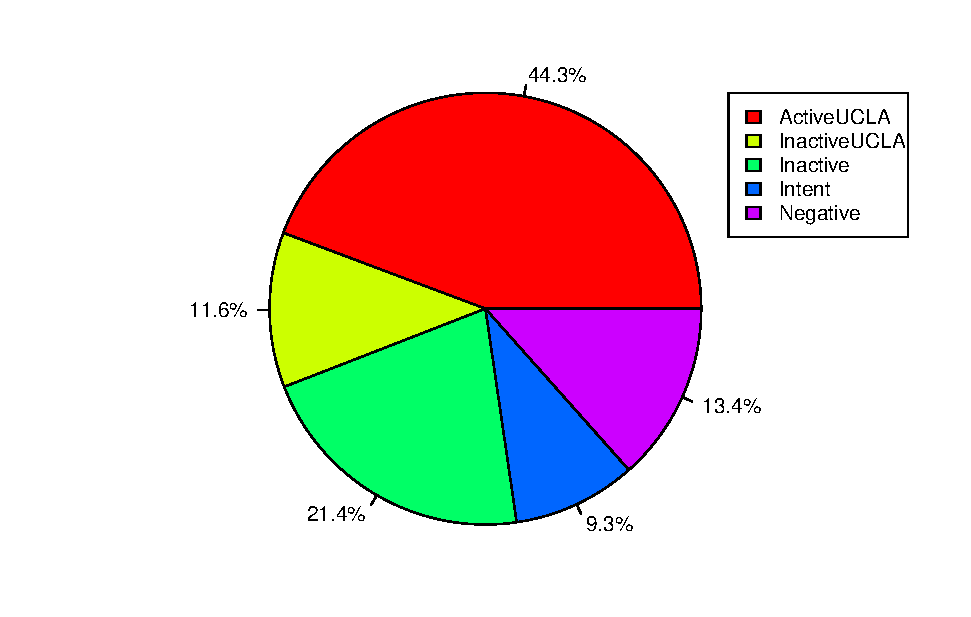
\includegraphics[width=0.5\textwidth]{experiment/uc.eps}
\caption{Manually user classification result.}
\label{fig:userclass}
\end{figure}

For active users, it is easy to see whether the user has related tweets about UCLA or photos about UCLA. For users without new tweets in recent two months, we call them inactive users and classify them according to Google result. We type their name with UCLA and see whether there is related search results.

\subsection{Intent mismatch}
The intent mismatch, labeled as ``Intent'' in Figure \ref{fig:userclass}, refers to the situations where the users are somehow related to UCLA but it is actually not belong to UCLA. The data show that intent mismatch often arises when a user follows a lot of UCLA users or a user talks about something that mentions UCLA.

There are several examples of intent mismatch. First, users may follow UCLA members in order to have more business opportunities, such as ``WeTutorLA'' and ``bombaybite''. The former one follows lot of students from UCLA, USC, UCSD and so on to let them noticed. The latter one follows a lot of organizations of UCLA because it is a restaurant near UCLA. Second, some users keeps follow back a lot of users, such as ``0neNiteStan''. This kind of users have a lot of tweets for advertisement. Third, users like ``USCTrojansNews'', ``openwestwood'' would ranked at higher position in our result. These users' tweets have significant intersection with users from UCLA. For example, ``USCTrojansNews'' often publish tweets that compare UCLA with USC while some users in UCLA category also like to do that. This makes our model make mistakes during the training process.

These kinds of intent mismatch contribute to $9.3\%$ discrepancies in the data. Typically, intent mismatch are very hard to be corrected since it requires human understanding of why this user may related to UCLA but not belongs to UCLA.

\subsection{Precision of active user}


\ifx \allfiles \undefined
\end{document}
\fi 

\section{Related Work}\label{sec:related-work}
abc

\cite{backstrom2011supervised}

\cite{elo1986rating}

\cite{kwak2010twitter}

\cite{welch2011topical}

\cite{wu2011says}

\cite{yang2011like}
\ifx \allfiles \undefined      
\documentclass{article}
\usepackage{booktabs}
\usepackage{multirow}
\usepackage{graphicx}
\usepackage{subfigure}

\begin{document}
\title{Conclusion}
\maketitle \else \fi

\section{Conclusion}\label{sec:conclusion}
Effectively estimating user profile and accordingly recommending service or suggesting friends are fundamental to all social networks. In this report, we have shown that the user's short bio is highly related to user's friendship and user's tweets. We presented three simple ranking approaches and a co-training framework that leverage both friendship and tweets evidence to solve the task purposed in our report. The graph approach analysis user profile from his followings and followers since that similar users are more likely to connected with each other. The Bayes approach extract the semantics of individual message that allow for the generation of user profile information of a given concept. Given the co-training framework, it is easy for us to combine two different approaches and obtain a better ranking result with limited positive training examples. The experiments results on twitter social network demonstrate that simple algorithms perform very well for our task. From the discussion, we learned the pros and cons of different approaches.

The co-training framework that combines graph information and tweets information are not limited to predict user hidden profiles, and can be applied to many other problems that require learning to rank nodes in a graph. There are some interest future research directions: First, the users are equally important in our model based on graph structure. However, we find many inactive users during our labeling process. We may assume users have different weight during the training process. Thus, there may exists the underlying mechanism of how the interactions and information between users related to their personal profile. Second, it is interesting to apply our algorithms in friends recommendation system. Currently, most friend recommendation systems were based on number of users' mutual friends. The co-training approach could leverage users' mutual friends information and other users' behavior such as tweets, profile. I think it is very helpful for building such framework for friends recommendation.

\ifx \allfiles \undefined
\end{document}
\fi


{\bibliography{twitter} \bibliographystyle{plain}}
\end{document}
